\let\negmedspace\undefined
\let\negthickspace\undefined
\documentclass[journal]{IEEEtran}
\usepackage[a5paper, margin=10mm, onecolumn]{geometry}
\usepackage{lmodern} % Ensure lmodern is loaded for pdflatex
\usepackage{tfrupee} % Include tfrupee package

\setlength{\headheight}{1cm} % Set the height of the header box
\setlength{\headsep}{0mm}     % Set the distance between the header box and the top of the text

\usepackage{gvv-book}
\usepackage{gvv}
\usepackage{cite}
\usepackage{amsmath,amssymb,amsfonts,amsthm}
\usepackage{algorithmic}
\usepackage{graphicx}
\usepackage{textcomp}
\usepackage{xcolor}
\usepackage{txfonts}
\usepackage{listings}
\usepackage{enumitem}
\usepackage{mathtools}
\usepackage{gensymb}
\usepackage{comment}
\usepackage[breaklinks=true]{hyperref}
\usepackage{tkz-euclide} 
\usepackage{listings}
% \usepackage{gvv}                                        
\def\inputGnumericTable{}                                 
\usepackage[latin1]{inputenc}                                
\usepackage{color}                                            
\usepackage{array}                                            
\usepackage{longtable}                                       
\usepackage{calc}                                             
\usepackage{multirow}                                         
\usepackage{hhline}                                           
\usepackage{ifthen}                                           
\usepackage{lscape}
\begin{document}

\bibliographystyle{IEEEtran}
\vspace{3cm}

\title{1.8.11}
\author{EE24BTECH11019 - DWARAK A}
% \maketitle
% \newpage
% \bigskip
{\let\newpage\relax\maketitle}

\renewcommand{\thefigure}{\theenumi}
\renewcommand{\thetable}{\theenumi}
\setlength{\intextsep}{10pt} % Space between text and floats


\numberwithin{equation}{enumi}
\numberwithin{figure}{enumi}
\renewcommand{\thetable}{\theenumi}


\textbf{Question}:

Find a relation between $x$ and $y$ such that the point \brak{x, y} is equidistant from the point \brak{3, 6} and \brak{-3, 4}.

\textbf{Solution: }
\begin{table}[h!]    
  \centering
  \begin{tabular}[12pt]{ |c|c|c|}
    \hline
	\textbf{Variable} & \textbf{Description} & \textbf{Value} \\ 
    \hline
    $\angle B$ & Angle at vertex $\vec{B}$ & $45\degree$ \\
    \hline 
    $\angle C$ & Angle at vertex $\vec{C}$ & $120\degree$ \\
    \hline
    $K=a+b+c$ & Perimeter of $\triangle\vec{ABC}$ & $10.4cm$ \\
    \hline
\end{tabular}

  \caption{Variables Used}
  \label{tab1.8.11.1}
\end{table}

If $\vec{X}$ is equidistant form the points $\vec{A}$ and $\vec{B}$

\begin{align}
	\norm{\vec{X}-\vec{A}}&=\norm{\vec{X}-\vec{B}} \label{eq1.8.11.1}\\
	\norm{\vec{X}-\vec{A}}^2&=\norm{\vec{X}-\vec{B}}^2 \label{eq1.8.11.2}\\
	\norm{\vec{X}}^2-2\vec{X}^\top\vec{A}+\norm{\vec{A}}^2&=\norm{\vec{X}}^2-2\vec{X}^\top\vec{B}+\norm{\vec{B}}^2\label{eq1.8.11.3}\\
	\brak{\vec{A}-\vec{B}}^\top\vec{X}&=\frac{\norm{\vec{A}}^2-\norm{\vec{B}}^2}{2} \label{eq1.8.11.4}
\end{align}

The above equation \ref{eq1.8.11.4} is the general expression for the perpendicular bisecting plane between any points $\vec{A}$ and $\vec{B}$.

Substituting the $\vec{A}$ and $\vec{B}$ values in the derived equation.

\begin{align}
	\myvec{6 \\ 2}^\top\vec{X} = \frac{\norm{\myvec{3 \\ 6}}^2-\norm{\myvec{-3 \\ 4}}^2}{2}=\frac{20}{2}=10\label{eq1.8.11.5}
\end{align}

Comparing with $n^\top x=c$

\begin{align}
	n=\myvec{6 \\ 2}\label{eq1.8.11.6}\\
	c=10
\end{align}

Line equation :

\begin{align}
	6x+2y=10 \label{eq1.8.11.7}
\end{align}

Final line equation :

\begin{align}
	3x+y=5 \label{eq1.8.11.8}
\end{align}

\begin{figure}[h!]
   \centering
   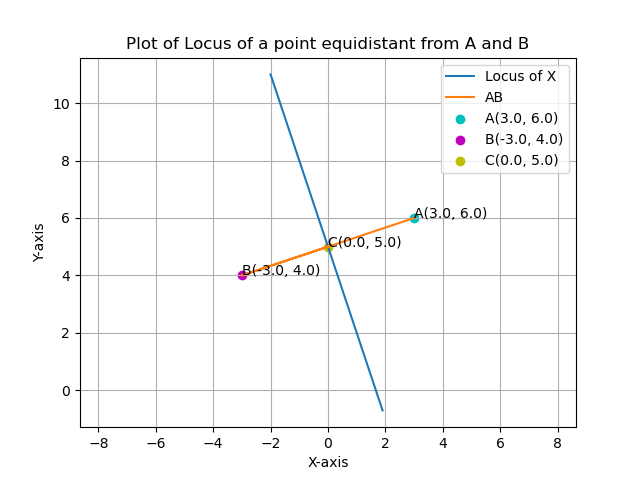
\includegraphics[width=0.8\linewidth]{figs/plot.png}
   \caption{Plot of point $\vec{X}$, equidistant from $\vec{A}$ and $\vec{B}$}
\label{stemplot}
\end{figure}
\end{document}
\end{document}
